\section{Four 4-transpositions}

\begin{theorem}
  There is a single sggi of rank 4 over $A_{11}$ that is composed by 4-transposition. This sggi is represented in the appendix~\ref{rank4-4-4transpositions} (p. \pageref{rank4-4-4transpositions})
\end{theorem}

\begin{proof}

  \paragraph{}
  Here is the common graph with the involutions $\rho_1$

  \begin{figure}[H]
    \begin{center}
      \begin{tikzpicture}

        \begin{scope}[every node/.style={circle,draw}]
          \node (1)  at (0,0)  {};
          \node (2)  at (2,0)  {};
          \node (3)  at (4,0)  {};
          \node (4)  at (6,0)  {};
          \node (5)  at (8,0)  {};
          \node (6)  at (10,0)  {};
          \node (7)  at (12,0)  {};
          \node (8)  at (14,0)  {};
          \node (9)  at (16,0)  {};
          \node (10) at (18,0)  {};
          \node (11) at (20,0) {};
        \end{scope}

        \begin{scope}[every node/.style={fill=white}]

          \begin{scope}[every edge/.style={draw}]
            \path (1)  edge node {$1$} (2);
            \path (3)  edge node {$1$} (4);
            \path (5)  edge node {$1$} (6);
            \path (7)  edge node {$1$} (8);
          \end{scope}
        \end{scope}

      \end{tikzpicture}
      \caption{}
    \end{center}
  \end{figure}

  \paragraph{}
  Ensuite, il nous faut rajouter l'involution $\rho_3$, comme d'habitude nous avons le choix entre trois possibilités : un carré alterné, deux doublements ou un doublement et relier deux points fixes. Nous ne pouvons pas utiliser de deux doublements car cela nous bloquerait (TODO). De même pour deux carrés alternés (TODO aussi).

  \paragraph{}
  Nous devons donc utiliser un carré alterné, un doublement et relier deux points fixes. On obtient

  \begin{figure}[H]
    \begin{center}
      \begin{tikzpicture}

        \begin{scope}[every node/.style={circle,draw}]
          \node (1)  at (0,2)  {};
          \node (2)  at (0,0)  {};
          \node (3)  at (2,2)  {};
          \node (4)  at (2,0)  {};
          \node (5)  at (4,2)  {};
          \node (6)  at (4,0)  {};
          \node (7)  at (6,2)  {};
          \node (8)  at (6,0)  {};
          \node (9)  at (8,2)  {};
          \node (10) at (8,0)  {};
          \node (11) at (10,2) {};
        \end{scope}

        \begin{scope}[every node/.style={fill=white}]

          \begin{scope}[every edge/.style={draw}]
            \path (1)  edge node {$1$} (2);
            \path (3)  edge node {$1$} (4);
            \path (5)  edge[bend right=20] node {$1$} (6);
            \path (7)  edge node {$1$} (8);
            \path (1)  edge node {$3$} (3);
            \path (2)  edge node {$3$} (4);
            \path (5)  edge[bend left=20] node {$3$} (6);
            \path (9)  edge node {$3$} (10);
          \end{scope}
        \end{scope}

      \end{tikzpicture}
      \caption{}
    \end{center}
  \end{figure}


  \paragraph{}
  Essayons maitenant de placer l'involution $\rho_0$. Cette involution doit commuter avec $\rho_3$, on a donc les mêmes contraintes que ci-dessus et elle doit former exactement un carré alterné, un doublement d'arête et relier deux points fixés par $\rho_3$. Les deux carrés doivent être adjacents sinon nous n'avons plus de place pour l'involution $\rho_2$. De plus le carré doit utiliser l'arête double précédemment formée et, par symmétrie, l'arête double qu'il forme doit être dans le carré créé à l'étape précédente (TODO). On a donc

  \begin{figure}[H]
    \begin{center}
      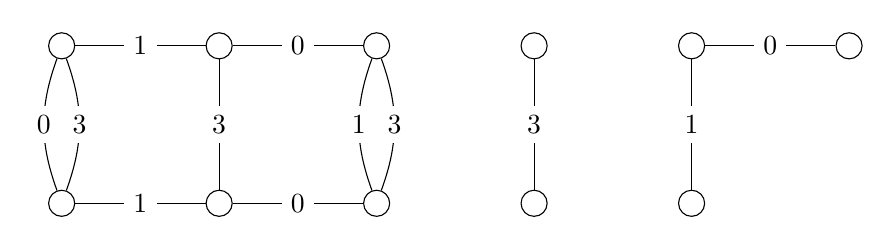
\begin{tikzpicture}

        \begin{scope}[every node/.style={circle,draw}]
          \node (1)  at (0,2)  {};
          \node (2)  at (2,2)  {};
          \node (3)  at (0,0)  {};
          \node (4)  at (2,0)  {};
          \node (5)  at (4,2)  {};
          \node (6)  at (4,0)  {};
          \node (7)  at (8,2)  {};
          \node (8)  at (8,0)  {};
          \node (9)  at (6,2)  {};
          \node (10) at (6,0)  {};
          \node (11) at (10,2) {};
        \end{scope}

        \begin{scope}[every node/.style={fill=white}]

          \begin{scope}[every edge/.style={draw}]
            \path (2)  edge node {$0$} (5);
            \path (4)  edge node {$0$} (6);
            \path (1)  edge[bend right=20] node {$0$} (3);
            \path (7)  edge node {$0$} (11);
            \path (1)  edge node {$1$} (2);
            \path (3)  edge node {$1$} (4);
            \path (5)  edge[bend right=20] node {$1$} (6);
            \path (7)  edge node {$1$} (8);
            \path (1)  edge[bend left=20] node {$3$} (3);
            \path (2)  edge node {$3$} (4);
            \path (5)  edge[bend left=20] node {$3$} (6);
            \path (9)  edge node {$3$} (10);
          \end{scope}
        \end{scope}

      \end{tikzpicture}
      \caption{}
    \end{center}
  \end{figure}

  \paragraph{}
  Maintenant il nous faut ajouter l'involution $\rho_2$ qui doit commuter avec $\rho_0$ de telle sorte que ce graphe soit transitif. Commençons par remarquer qu'il est impossible de raccorder directement l'arête $\rho_3$ isolée sur les deux carrés alternés. En effet, vu que nous sommes obligés d'utiliser $\rho_2$, nous ne pouvons pas utiliser les deux points centraux car ils sont connectés à une arête $\rho_0$ et il n'est pas possible de former de carré car nous aurions utilisé nos 4 arêtes et le graphe ne serait pas transitif. De même, nous ne pour l'arête double avec $\rho_0$. Pour l'arête double avec $\rho_1$, ces sommets sont adjacents à des arêtes $\rho_1$ donc c'est aussi impossible.

  \paragraph{}
  Il faut donc raccoder, dans l'ordre, les carrés adjacent aux deux arêtes $\rho_1$ et $\rho_2$ puis raccorder ceci à l'arête $\rho_3$. Dans le premier raccordement, nous devons former un carré alterné avec les arêtes $\rho_2$. Ce qui nous donne le graphe suivant.

  \begin{figure}[H]
    \begin{center}
      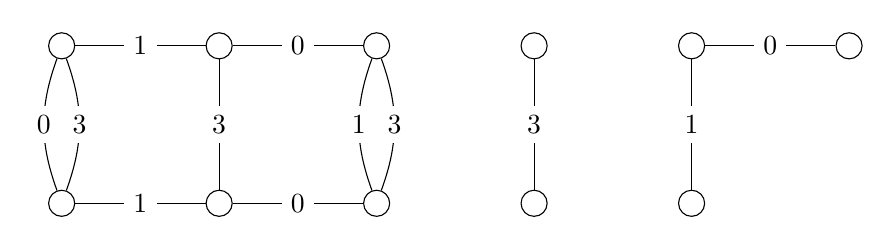
\begin{tikzpicture}

        \begin{scope}[every node/.style={circle,draw}]
          \node (1)  at (0,2)  {};
          \node (2)  at (2,2)  {};
          \node (3)  at (0,0)  {};
          \node (4)  at (2,0)  {};
          \node (5)  at (4,2)  {};
          \node (6)  at (4,0)  {};
          \node (7)  at (8,2)  {};
          \node (8)  at (8,0)  {};
          \node (9)  at (6,2)  {};
          \node (10) at (6,0)  {};
          \node (11) at (10,2) {};
        \end{scope}

        \begin{scope}[every node/.style={fill=white}]

          \begin{scope}[every edge/.style={draw}]
            \path (2)  edge node {$0$} (5);
            \path (4)  edge node {$0$} (6);
            \path (1)  edge[bend right=20] node {$0$} (3);
            \path (7)  edge node {$0$} (11);
            \path (1)  edge node {$1$} (2);
            \path (3)  edge node {$1$} (4);
            \path (5)  edge[bend right=20] node {$1$} (6);
            \path (7)  edge node {$1$} (8);
            \path (1)  edge[bend left=20] node {$3$} (3);
            \path (2)  edge node {$3$} (4);
            \path (5)  edge[bend left=20] node {$3$} (6);
            \path (9)  edge node {$3$} (10);
          \end{scope}
        \end{scope}

      \end{tikzpicture}
      \caption{}
    \end{center}
  \end{figure}


\end{proof}
